\section{Component Implementation Description}
\label{sec:ComponentImplementation}

In general, a component model does not provide any information about the inner
structure of its components, since components are regarded as a black-box
entities. However, black-box components inhibit the analysis of Quality of
Service (QoS) attributes of the system, since important information about the
dependency of these attributes on external services, hardware and software
resources, and the usage profile cannot be specified.  With black-box
components, only static QoS contracts, like the ones specified by the QoS
Modelling Language (QML) \cite{frolund1998a}, can be used, but these are not
sufficient for this task. If the required QoS profile of a component cannot be
provided by its environment, the component is likely to work, but with lower
quality. Therefore, we need additional information on the inner
structure to analyse QoS attributes of a component in dependence on its
environment at design time.

We state that a component can still be considered a black-box entity if the additional
information used by parametric contracts (a) does not expose intellectual
property of the component vendor and (b) has not to be understood by human
users. So, the additional information and its analysis has to be transparent
for the deployer. 

Parametric contracts \cite{reussner2002c} extend the design by contract principle of software components. The provided interfaces (postcondition) of a component are computed in dependence on the actual interfaces offered by the environment (precondition). The relationship between provided and required interfaces of a software component can be used to compute the influence of external services used by the component on its QoS attributes as well. We distinguish between \emph{basic components} and \emph{composite components} as two different ways of implementing a component.

\subsection{Basic Component}
A \emph{basic component} represents a basic block that is not further subdivided. It implements a certain functionality and is defined by its provided interfaces, required interfaces, and service effect specifications.

A \emph{service effect specification} describes the relationship between provided and required interfaces. It defines the externally visible behaviour of a provided service. This includes the used external services, possible call sequences, and, for example, probabilities of service calls. A service effect specification can be modelled in different ways. It can be a signature list that only contains the called external services. It can model all possible call sequences executed by a provided service. This can be expressed by different means, for example, finite state machines, Petri nets, regular expressions, or any other kind of grammar. In any case, a service effect specification is an abstraction of component source code. It models calls to external services only and neglects the internal component code.

\begin{figure}[htbp]
\centering
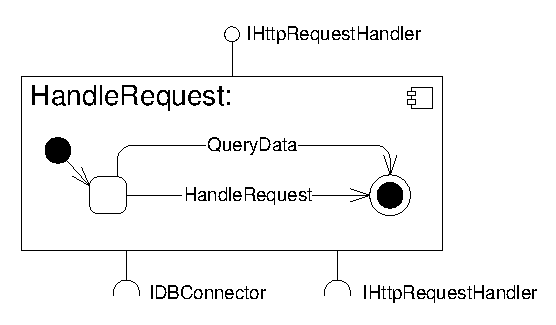
\includegraphics[scale=0.85]{example/HandleRequestSEFF}
\caption{Service effect specification of the method HandleRequest in the DynamicFileProvider.}
\label{fig:seff}
\end{figure}

Figure \ref{fig:seff} shows a simple service effect specification modelled as a finite state machine. If the method HandleRequest of the DynamicFileProvider is responsible for the incoming request it executes a query on the connected database. In the internal code that is not visible here, it creates the web page and returns the result to the client. If it is not responsible for the incoming request it forwards the request to the next component in the chain of responsibility. This is done by the call of the HandleRequest method of the component connected to the IHttpRequestHandler interface.

The fact that a basic component represents a single block does not imply that the real implementation hast to be one 'block' as well. Since we are talking about the implementation description and not the actual implementation, this difference is possible and actually desired in some cases. For example, the actual implementation of a component might consist of a set of classes and/or subcomponents. This information is abstracted away in the description as a basic component. So, the description of a basic component only represents one view on a software component. Another view on a component are, for example, a class diagram or its source code.

\subsection{Composite Component}
A \emph{composite component} consists of a set of interconnected subcomponents that
realise its functionality. 

An \emph{assembly connector} connects a required interface of an inner component to a provided interface
of another inner component. 

\emph{Delegation connectors} map provided and required
interfaces of the composite component to interfaces of its inner
structure. 

A provides delegation connector maps
a provided interface of the composite component to provided interface of an
inner component. 

A requires delegation connector maps a required interface of an
inner component to a required interface of the composite component.

The HttpRequestProcessor of the web server architecture.

As described in section \ref{sec:ComponentTypes}, a component implementation
conforms to a complete-type if it offers at least the functionality specified
in by the provided interfaces of the complete type and does not require more
functionality than specified in the required interfaces of the complete-type.

In section \ref{sec:ComponentTypes}, we introduced provided- and complete-types
of components. Is the component implementation description also a type? In
theory, there might exist different implementations that conform to the same
implementation description (see Model Driven Architectures, MDA
\cite{TODO:reference}). Hence, the implementation description would be a
type. However, the implementation of a component and its description is
usually in a one to one relationship. For this reason, we do not consider the
component implementation as a type. 

Figure \ref{fig:TypeHierarchy} gives an overview of the relation of
provided-types, complete-types and component implementation descriptions.
TODO:Figure and description

With the implementation description of software components, we have enough
information to compute QoS attributes of the component in dependence on external
services.
TODO:Example
